\documentclass[10pt,a4paper]{report}
\usepackage[utf8x]{inputenc}
\usepackage{ucs}
\usepackage{amsmath}
\usepackage{amsfonts}
\usepackage{amssymb}
\usepackage{graphicx}
\usepackage[english]{babel}

\usepackage{parskip}
\setlength{\parindent}{0cm}
\setlength{\marginparwidth}{2.5cm}
\setlength{\marginparsep}{0.5cm}

\usepackage{fancyhdr}
\pagestyle{fancy}
\fancyhead{}
\fancyhead[C]{\small{\textsc{ETemplate2 JavaScript Documentation}}}
\renewcommand{\headrulewidth}{0pt}


\title{ETemplate2 JavaScript Documentation}

\begin{document}

\chapter*{ETemplate2 JavaScript Documentation}

\section*{Abstract}

In contrast to our last approach, the new \textit{ETemplate2}-System renders the ETemplate templates completely on the client. When a template should be displayed, the URL to the template definition XET file, plus the initial content array is sent to the client. The client downloads the XET file (most of the time it will come from the browser cache), parses and renders it and sets the values of the widget according to the ones defined in the content array.

\section*{JS Inheritance System}
Instead of using the jQuery-Class system as we did before, a new inheritance system has been introduced (see \textit{et2\_inheritance.js}). It features:
\begin{itemize}
	\item Basic class inheritance
	\item Support for interfaces
	\item Support for attributes
\end{itemize}

\subsection*{Basic inheritance}

To create a class write
\begin{verbatim}
var MyClass = Class.extend([interfaces, ] functions/attributes);
\end{verbatim}
where ``interfaces'' is a single interface or an array of interfaces (see below) and functions/attributes an object containing the functions the class implements. You can extend \textit{MyClass} again by writing
\begin{verbatim}
var MyOtherClass = MyClass.extend([interfaces, ]
                       functions/attributes);
\end{verbatim}
The \textit{extend} function only extends the prototype and is only run once, when the JS file is intially parsed. Creating classes using the inheritance system introduces nearly no additional speed impact.

\subsection*{Defining functions}

\paragraph{Simple functions:}
To define a function simply add it to the functions object:
\begin{verbatim}
var MyClass = Class.extend({
    myFunction: function(_param) {
    	console.log("myFunction has been " + 
    	    "called with param", param);
    }
});
\end{verbatim}

\paragraph{Override functions:}
To override functions in another class write:
\begin{verbatim}
var MyOtherClass = MyClass.extend({
    myFunction: function(_param1, _param2) {
        // If this._super is not found inside
        // the function, the code overhead for
        // overriding functions is not created
        this._super(_param1);
		
        console.log("And _param2 is ", _param2);
    }
});
\end{verbatim}

\paragraph{Constructor and destructor:}
The constructor function is named ``\textit{init}''. It underlies the same overriding-mechanism as all other functions. When overriding the init function it is the best (as it probably is with all other functions too) to call the inherited super function with
\begin{verbatim}
this._super.apply(this, arguments);
\end{verbatim}
The destructor is not really part of the inheritance system but used inside the widget system. The destructor is named ``\textit{destroy}'' and should \textsc{always} be written in order to free all references to other objects, delete all DOM-Nodes and unbind all event handers. When deriving from some higher-level widget classes it will be enough to override the ``detatchFromDOM'' method and sometimes even to do nothing (see below).


\subsection*{Interfaces}

\paragraph{Using interfaces:}
Interfaces can be used to check whether a class implements a certain set of functions. You can create an interface declaration by writing something like:
\begin{verbatim}
var IBreathingObject = new Interface({
    breath: function() {}
});
\end{verbatim}
The construct with the empty function is only to make the interface declaration look syntactically pleasing, other objects are not allowed inside the interface declaration.

To make a class extending a interface simply write
\begin{verbatim}
var MyClass = new Class.extend([IBreathingObject, ...], {
    [...]
});
\end{verbatim}
or in the case of only one interface
\begin{verbatim}
var MyClass = Class.extend(IBreathingObject, {
    [...]
});
\end{verbatim}
If a class does not implement all functions declared in the interface, it is marked as \textit{abstract} and an attempt on creating it will throw an exception.

\paragraph{Extended type check:}
You can check whether a class/object derrives from a certain interface by using the \textit{implements} function (\textit{implements} does \textsc{not} check whether the functions are really implemented, just whether the class/object has been defined with that interface.

Example:
\begin{verbatim}
var MyClass = Class.extend(IBreathingObject, {
	[...]
});

MyClass.prototype.implements(IBreathingObject); // true

var obj = new MyClass();
obj.implements(IBreathingObject); // true
\end{verbatim}

\textit{Implements} only checks for interfaces - if you want to check whether an object is instance of another class or implements a certain interface, you can use the \textit{instanceOf} function. In the above example:
\begin{verbatim}
obj.instanceOf(Class); // true
obj.instanceOf(MyClass); // true;
obj.instanceOf(IBreathingObject); // true
\end{verbatim}


\subsection*{Attributes}

\paragraph{Basic usage:}
Attributes are used to declare a certain set of variables, getters and setters which are automatically used when (de-)serializing the object. Additionally the attributes can be used to add some documentation and type safety to the classes. To define attributes, simply add an ``attribute''-object to your class definition:
\begin{verbatim}
var MyClass = Class.extend({
    attributes: {
        "color": {
            "name": "Color",
            "type": "string",
            "default": "red",
            "description": "This is just an example"
        }
    }
});
\end{verbatim}

\paragraph{Default attribute values:}
When the object is created, after the "init" functions have been called, the default value of the attribute will be set, without overriding existing object-variables which have the same name as the attribute. If no default is given, the default value defaults to an default value defined for the given type. The type defaults to ``any'' which means, that no type-check is done (see Table \ref{tbl:attr_types}). If you do not wish the default value to be automatically set, set the default value to the ``et2\_no\_default'' object.

\begin{table}
	\begin{center}
		\begin{tabular}{r | l l}
			 & \textbf{default value} & \textbf{special conversions} \\
			\hline
			string & \texttt{""} & \\
			integer & \texttt{0} & strings are parsed to ints \\
			floats & \texttt{0.0} & strings are parsed to floats \\
			boolean & \texttt{false} & the strings \texttt{"false"}, \texttt{"true"}, and \texttt{""} \\
			any & \texttt{null} & \\
		\end{tabular}
	\end{center}
	\label{tbl:attr_types}
	\caption{Overview over all available attribute types, their standard default values and special conversions}
\end{table}

\paragraph{Setters and getters:}
You can manually \textit{set} an attribute by calling the function
\begin{verbatim}
obj.setAttribute(name, value);
\end{verbatim}
\texttt{setAttribute} checks for the existance of the attribute with the given name and typechecks the given value. When setting an attribute, the code checks, whether a setter function named ``\texttt{set\_[name]}'' is found. If yes, the function is called with the given value as parameter. If the function does not exist, the following code is executed
\begin{verbatim}
obj[name] = value;
\end{verbatim}

You can manually \textit{get} an attribute by calling the function
\begin{verbatim}
obj.getAttribute(name);
\end{verbatim}
Just like the \texttt{setAttribute} function, \texttt{getAttribute} searches for a getter function named ``\texttt{get\_[name]}'' first and simply returns \texttt{obj[name]} if the getter function is not found.

\paragraph{Ignoring attributes:}
Sometimes you may want the \texttt{setAttribute} function to simply ignore a certain attribute - in ETemplate2 for example, the \textit{span} attribute is ignored, as it is read by the grid class. To mark an attribute as ``ignored'' simply add:
\begin{verbatim}
"ignore": true
\end{verbatim}
to the attribute definition. Setting an attribute to be ignored can also be done at runtime - but this only effects objects of exactly the same class, as attribute definitions are copied between prototypes and not referenced.

\paragraph{Attribute inheritance:}
All classes automatically inherit the attributes of their parent class. You can change the attribute definition for a new class by simply defining a new entry for it. The entry can also be partial. So in our above example, we could simply change the color-attribute to be an integer value, as e.g. the new class directly uses the binary-representation of the color:
\begin{verbatim}
var MyOtherClass = MyClass.extend({
    attributes: {
        "color": {
            "type": "integer"
        }
    }
});
\end{verbatim}

\paragraph{JS Dependencies:}
The JS dependency management is done on the server-side by EGW, so it cannot be used or tested when using the standalone test method (see below). However, you can mark dependencies by using the
\begin{verbatim}
/*egw:uses
    jquery.jquery;
    et2_baseWidget;
*/
\end{verbatim}
syntax. Note that this comment has to start in the first 16 lines. More information on that topic can be found in the preamble of 

\begin{center}\texttt{class.egw\_include\_mgr.inc.php}\end{center}

in phpgwapi.


\section*{ETemplate2 class structure}

\subsection*{Overview}
The following UML class diagram (see figure \ref{fig:uml}) gives an overview over the \textit{ETemplate2} class structure. Basically the widgets form a tree and when loading the XET-file, the widget objects are automatically created according to the XML-Tag. Widget classes can be registered using the
\begin{verbatim}
et2_register_widget(class_prototype, array_of_tagnames);
\end{verbatim}
function.

\begin{figure}
	\begin{center}
		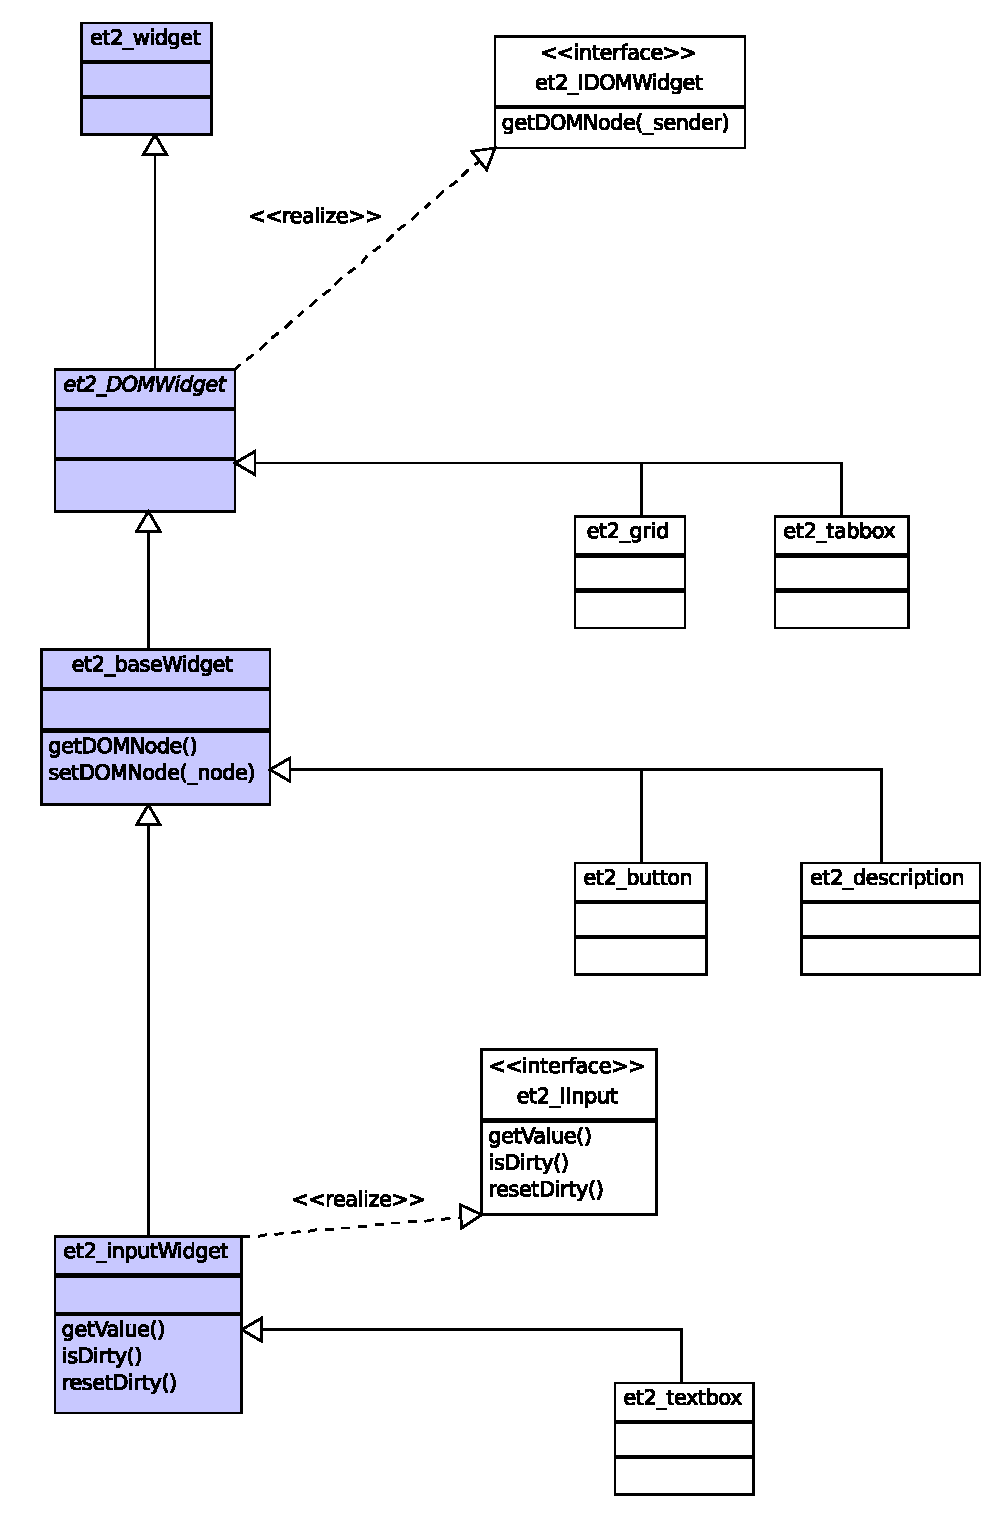
\includegraphics[scale=0.6]{media/class_structure.pdf}
	\end{center}
	\caption{Overview over the ETemplate2 JavaScript side class structure. The blue classes are the ones you normally derrive other classes from.}
	\label{fig:uml}
\end{figure}

\subsection*{et2\_widget}

\paragraph{Overview:}
\textit{et2\_widget} is the base widget class. It spans the widget tree and introduces features for managing the child widgets, like adding and destryoing them. The constructor takes to parameters, the parent and the actual tag name the widget was created for. The tag name is stored in the ``type'' object-variable. The widget automatically adds itself to the parent children list and removes itself from the list when it is destroyed.

\paragraph{XML-Handling:}
\textit{et2\_widget} has three important functions for XML handling:
\begin{verbatim}
et2_widget::loadFromXML(_node)
\end{verbatim}
Reads the attributes for this widget from the given XML-DOM-Node. All child widgets are created and the LoadFromXML-function is recursively called for them.

\begin{verbatim}
et2_widget::loadAttributes(_attrs)
\end{verbatim}
Is called by \texttt{LoadFromXML} with the XML-DOM-Attributes object. The base implementation simply calls the ``\texttt{setAttribute}'' function for every attribute found.

\begin{verbatim}
et2_widget::loadContent(_text)
\end{verbatim}
Is called whenever \texttt{loadFromXML} finds a text-node inside the XML data. The base implementation does nothing when reaching a text node.

\paragraph{Cloning widgets:}
\textit{et2\_widget} introduces a mechanism which can be used to clone widgets and to assign the attributes of other widgets to them. The clone function
\begin{verbatim}
et2_widget::clone(_parent);
\end{verbatim}
takes the parent widget the cloned widget should be added to.

\paragraph{Updating the widget:}
\textit{et2\_widget} has a function called \texttt{update} which reads all attributes and setts them again.
\begin{verbatim}
et2_widget::update()
\end{verbatim}
This function is e.g. important if you replace the DOM-Node of a widget (see below) and want to call all attribute setters. The \texttt{upate} function does that automatically.

\subsection*{et2\_IDOMNode interface}
The \textit{et2\_IDOMNode} interface declares the
\begin{verbatim}
et2_IDOMNode::getDOMNode(_sender)
\end{verbatim}
function, which has to be implemented by all widgets which have a representation in the HTML-DOM-Tree. \texttt{getDOMNode} should return the DOM-Node of the current widget. The return value has to be a plain DOM node, not a jQuery object. The \texttt{\_sender} parameter defines which widget is asking for the DOMNode. Depending on that, the widget may return different nodes. This is used in the grid or the tab. Normally the \_sender parameter can be omitted in most implementations of the getDOMNode function. However, you should always provide the \texttt{\_sender} parameter when calling \texttt{getDOMNode}!

\subsection*{et2\_DOMWidget}
The \textit{et2\_DOMWidget} class is derrived from \textit{et2\_IDOMNode} and \textit{et2\_widget} without implementing the \texttt{getDOMNode} funcition. It  introduces an mechanism which automatically inserts the DOM-Node of this widget into the DOM-Node of the parent widget (if the parent widget implements \textit{et2\_IDOMWidget}. The two functions
\begin{verbatim}
et2_DOMWidget::attachToDOM()
et2_DOMWidget::detatchFromDOM()
\end{verbatim}
have to be extended by any class which derrives from \textit{et2\_DOMwidget} and attaches event-handlers to the DOM. All event handlers have to be detached in the \texttt{detatchFromDOM} function and (re-)attached in the \texttt{attachToDOM} function. See the \textit{et2\_baseWidget} statustext-code for an example. The \textit{et2\_DOMWidget} also automatically sets the \textit{id} property of its DOM-Node.

Directly derrive a widget from the \textit{et2\_DOMWidget} class, if you have to return different DOM-Nodes depending on the widget which asked for the DOM-Node and therefore need an own implementation of the \texttt{getDOMNode} function.

\subsection*{et2\_baseWidget}
\textit{et2\_baseWidget}, derrived from \textit{et2\_DOMWidget} is in most cases the best choice whe implementing an widget. It introduces the function
\begin{verbatim}
et2_DOMWidget::setDOMNode(_node)
\end{verbatim}
and implements \texttt{getDOMNode}. Calling \texttt{setDOMNode} detatches the current node from the DOM-Tree and attaches the given node. Very basic widgets only have to call \texttt{setDOMNode} once in the constructor. Widgets which can change their underlying DOM-Node can call \texttt{setDOMNode} e.g. from setter functions. Remember that you have to reapply all changes you've made to the DOM-Node, so probably you'll have to call \texttt{update()} after having set the new DOM-Node.

\subsection*{et2\_IInput Interface}
\textit{et2\_IInput} is the base interface for all widgets which can return a value. The three functions, which have to be implemented are rather self-explanatory:
\begin{verbatim}
et2_IInput::getValue()
et2_IInput::isDirty()
et2_IInput::resetDirty()
\end{verbatim}

\subsection*{et2\_inputWidget}
The \textit{et2\_inputWidget} derrives from \textit{et2\_baseWidget} and \textit{et2\_IInput}. This class automatically reads its content from the content-array when its id is set (behaviour might be changed). It has a function
\begin{verbatim}
et2_inputWidget::getInputWidget()
\end{verbatim}
which as a default returns the DOM-Node of the widget. In more complicated widgets where the base DOM-Node is not equally to the input-DOM-Node you can override this function.

The setters and getters for the value attribute of the widget utilize the jQuery ``\texttt{val()}'' function for the DOM-Node returned by
\begin{verbatim}
et2_inputWidget::getInputWidget()
\end{verbatim}

In some complicated cases it might be better not to derrive directly from \texttt{et2\_inputWidget} but from \texttt{et2\_baseWidget} or even \texttt{et\_DOMWidget} and simply implement \texttt{et2\_IInput}.

\section*{Conventions and testing}

New widgets should be in their own JS-File named like the widget. They can by easily tested by including the JS-File in \texttt{test\_xml.html} found in the ``test'' folder. You can simply add new tests using the same scheme as with the existing tests.

Please \textsc{always} test, whether your widget also works properly if it is wrapped in a template, as this causes the widget to be cloned, which creates a completely different situation in comparison to reading the widget directly from XML. A test XET-File for this may look like that:
\begin{verbatim}
<overlay>
    <!-- Test without template -->
    <mywidget/>
    
    <!-- Test with template -->
    <template id="test">
        <mywidget/>
    </template>
    <!-- Reference the template above -->
    <template id="test"/>
</overlay>
\end{verbatim}

There are also many more or less helpfull debug messages in the code. You can regulate the amout of messages by setting the \texttt{ET2\_DEBUGLEVEL} variable in \textit{et2\_common.js}.

\end{document}